% ============================================================================
%  KAVACH AI - Project Review Documentation
%  Compile with pdfLaTeX (works out of the box on Overleaf).
%
%  FILL IN YOUR DETAILS: edit the \newcommand values in the "Project details"
%  block below (team members, institution, department, guide, date).
% ============================================================================
\documentclass[11pt,a4paper]{article}

% ---------- Packages ----------
\usepackage[T1]{fontenc}
\usepackage[utf8]{inputenc}
\usepackage{lmodern}
\usepackage[margin=1in]{geometry}
\usepackage{graphicx}
\usepackage{booktabs}
\usepackage{longtable}
\usepackage{array}
\usepackage{enumitem}
\usepackage{titlesec}
\usepackage{fancyhdr}
\usepackage{xcolor}
\usepackage{listings}
\usepackage{amssymb}
\usepackage{tikz}
\usetikzlibrary{arrows.meta,positioning,shapes.geometric,fit,backgrounds,calc}
\usepackage[hidelinks]{hyperref}
\usepackage{caption}

% ---------- Project details (EDIT THESE) ----------
\newcommand{\projectname}{KAVACH AI}
\newcommand{\projecttagline}{Local-First Document Intelligence Workbench}
\newcommand{\teamname}{Project Team}
\newcommand{\memberA}{Member 1 (Roll No.)}
\newcommand{\memberB}{Member 2 (Roll No.)}
\newcommand{\memberC}{Member 3 (Roll No.)}
\newcommand{\memberD}{Member 4 (Roll No.)}
\newcommand{\institution}{Institute Name}
\newcommand{\department}{Department of Computer Science and Engineering}
\newcommand{\guidename}{Project Guide}
\newcommand{\reviewdate}{\today}

% ---------- Colors (field-manual palette) ----------
\definecolor{ink}{HTML}{202923}
\definecolor{oxide}{HTML}{C94F30}
\definecolor{forest}{HTML}{3F7051}
\definecolor{paper}{HTML}{F2EFE6}
\definecolor{linec}{HTML}{C9C3B5}
\definecolor{danger}{HTML}{B73D2B}

% ---------- Section styling ----------
\titleformat{\section}{\normalfont\Large\bfseries\color{ink}}{\thesection}{0.6em}{}
\titleformat{\subsection}{\normalfont\large\bfseries\color{ink}}{\thesubsection}{0.6em}{}
\titleformat{\subsubsection}{\normalfont\normalsize\bfseries\color{oxide}}{\thesubsubsection}{0.6em}{}
\titlespacing*{\section}{0pt}{14pt}{6pt}
\titlespacing*{\subsection}{0pt}{10pt}{4pt}

% ---------- Header / footer ----------
\pagestyle{fancy}
\fancyhf{}
\fancyhead[L]{\small\color{ink!75}\projectname\ -- Project Review}
\fancyhead[R]{\small\color{ink!75}\thepage}
\renewcommand{\headrulewidth}{0.4pt}
\renewcommand{\headrule}{\hbox to\headwidth{\color{oxide}\leaders\hrule height \headrulewidth\hfill}}

% ---------- Listings ----------
\lstdefinestyle{code}{
  basicstyle=\ttfamily\footnotesize,
  backgroundcolor=\color{paper},
  frame=single,
  rulecolor=\color{linec},
  breaklines=true,
  columns=fullflexible,
  keepspaces=true,
  showstringspaces=false,
  keywordstyle=\color{oxide}\bfseries,
  commentstyle=\color{forest!85!black}\itshape,
  stringstyle=\color{ink},
  numbers=left,
  numberstyle=\tiny\color{ink!50},
  numbersep=8pt,
}
\lstset{style=code}

% ---------- TikZ styles ----------
\tikzset{
  layer/.style={draw=ink!55, fill=paper, rounded corners=2pt,
                minimum width=13.4cm, minimum height=1.0cm, align=center, font=\small},
  stage/.style={draw=ink!55, fill=paper, rounded corners=2pt,
                minimum width=4.8cm, minimum height=8.5mm, align=center, font=\small},
  box/.style={draw=ink!55, fill=paper, rounded corners=2pt,
              minimum height=9mm, align=center, font=\small},
  arrow/.style={-{Stealth[length=2.2mm]}, draw=ink!70, thick},
  oarrow/.style={-{Stealth[length=2.2mm]}, draw=oxide, thick},
  note/.style={draw=oxide!70, fill=oxide!7, rounded corners=2pt, align=left, font=\scriptsize, inner sep=5pt},
}

\begin{document}

% ============================================================================
% TITLE PAGE
% ============================================================================
\begin{titlepage}
\centering
\vspace*{1.2cm}

{\color{oxide}\rule{0.82\textwidth}{1.6pt}}\\[0.5cm]
{\Huge\bfseries\color{ink} \projectname}\\[0.35cm]
{\Large\color{ink!80} \projecttagline}\\[0.35cm]
{\color{oxide}\rule{0.82\textwidth}{1.6pt}}\\[1.6cm]

{\large\bfseries Project Review Documentation}\\[0.3cm]
{\large Submitted in partial fulfilment of the project review requirements}\\[1.8cm]

{\large\bfseries Submitted by}\\[0.4cm]
\begin{tabular}{c}
\memberA \\[2pt]
\memberB \\[2pt]
\memberC \\[2pt]
\memberD \\
\end{tabular}\\[1.6cm]

{\large \department}\\[0.25cm]
{\large \institution}\\[1.6cm]

{\large Project Guide: \guidename}\\[1.8cm]

{\large \reviewdate}

\vfill
{\footnotesize\color{ink!60} This document describes a local document-analysis application. Use the post-optimization checklist before deployment.}
\end{titlepage}

% ============================================================================
% ABSTRACT
% ============================================================================
\section*{Abstract}
\addcontentsline{toc}{section}{Abstract}

Industrial and government organisations produce large volumes of confidential
knowledge work --- inspection reports, equipment manuals, engineering
calculations, Piping and Instrumentation Diagrams (P\&IDs), internal code, and
vendor documents. This material cannot be sent to public cloud AI services,
which leaves organisations choosing between slow manual review and a
data-sovereignty breach. \projectname{} is a self-hosted, air-gapped workbench
that keeps the entire analysis pipeline on the organisation's own hardware.
A request is handled by a team of nine single-purpose agents: security
verification, task routing, document ingestion, vision, retrieval-augmented
generation (RAG), reasoning, verification, deliverable generation, and a
bounded agentic planner that decides which action runs next. Domain profiles
(General documents, Industrial engineering) select the review vocabulary, and
analysis modes (Risk review, Summary, Field extraction) select the task. Every
quoted excerpt is re-checked against its source, and high-risk, low-confidence,
or unsupported findings are held for human approval. Host development routes
inference to local Ollama models (\texttt{qwen3:8b}, \texttt{llava:7b},
\texttt{llama3.2:3b}, \texttt{nomic-embed-text}) with explicit model-availability errors; the System page reports real GPU telemetry through
\texttt{nvidia-smi} and CPU/RAM through \texttt{psutil}. The implementation is
validated by a 114-test backend suite covering the planner guardrails, the tool
allowlist, the review gate, model routing, document profiles and modes, and
uploaded-document analysis.

\medskip
\noindent\textbf{Keywords:} local-first AI, air-gapped inference, RAG,
agentic workflow, human-in-the-loop, document intelligence, Ollama.

\newpage
\tableofcontents
\newpage

% ============================================================================
% 1. INTRODUCTION
% ============================================================================
\section{Introduction}

\subsection{Background and Motivation}
Refineries, public-sector units, defence-linked manufacturers, and government
offices routinely handle documents whose disclosure is unacceptable. Cloud AI
services offer convenience but require transmitting the material outside the
organisation's boundary. The alternative --- fully manual review --- is slow,
inconsistent, and does not scale with document volume.

Local open-weight language models have reached a level where useful document
analysis can run on a single workstation GPU. \projectname{} builds on this
capability and treats it as an engineering system: every step of a run is
recorded, every finding cites its source, and a human reviewer remains the
final authority.

\subsection{Problem Statement}
Design and implement a self-hosted workbench that (i) analyses confidential
documents entirely on local hardware, (ii) produces findings with verifiable
source evidence rather than ungrounded model output, (iii) supports different
document domains through configurable profiles, and (iv) enforces a
human-in-the-loop approval gate for risky or uncertain results --- while
remaining auditable at every step.

\subsection{Objectives}
\begin{enumerate}[leftmargin=1.4em]
  \item Build a local-only agent pipeline for document analysis with no
        outbound AI calls.
  \item Provide domain profiles and selectable analysis modes (risk review,
        summary, field extraction).
  \item Ground findings in source text and automatically re-verify every
        quoted excerpt.
  \item Implement a bounded agentic planner with hard guardrails: step limit,
        loop detection, fixed tool allowlist, and a mandatory review gate.
  \item Expose the whole system through an operations console: workbench,
        document vault, knowledge base, run history, model router, security
        centre, deliverables, and live system status.
  \item Report measured values and explicit unavailable states; document deployment limits.
\end{enumerate}

\subsection{Scope}
The prototype targets text-readable documents (TXT, CSV, PY, DOCX, PDF) and
supports image description through a local vision model. It runs on a single
workstation (CPU or GPU) and does not require any cloud service. All analysis uses stored user documents; new installations contain no content.

% ============================================================================
% 2. BACKGROUND
% ============================================================================
\section{Background}

\subsection{On-Premise versus Cloud AI}
Cloud inference offers scale but violates data-residency requirements for
confidential industrial material. On-premise inference with open-weight models
removes the data-transfer problem; the trade-off is model size and hardware
cost, both of which have improved substantially with quantised 3B--8B models.

\subsection{Retrieval-Augmented Generation (RAG)}
RAG improves factuality by retrieving relevant passages from a local corpus and
supplying them as context. \projectname{} uses a lightweight in-memory index:
text is chunked, embedded locally, and ranked by cosine similarity. When Ollama
is available, embeddings are produced by \texttt{nomic-embed-text}; otherwise a
deterministic 256-dimensional hash embedding keeps the pipeline functional.

\subsection{Agentic Workflows and Guardrails}
An agentic system chooses its own next action instead of following a fixed
script. Because unbounded autonomy is unacceptable in an industrial context,
\projectname{} constrains the planner: it may only choose among eligible
actions, each backed by one allowlisted tool, with a step budget, loop
detection, and a review gate that always runs last.

\subsection{Local Inference Runtime}
Ollama provides a local HTTP runtime for open-weight models. In
\texttt{airgapped} mode, \projectname{} requires the Ollama endpoint to be
loopback (\texttt{localhost} / \texttt{127.0.0.1}); any other host raises an
air-gap violation.

% ============================================================================
% 3. SYSTEM ARCHITECTURE
% ============================================================================
\section{System Architecture}

\subsection{Overview}
\projectname{} is organised in five layers: the operations console, the HTTP
API, the agent orchestrator, the model providers, and local storage. No layer
communicates with an external service.

\begin{figure}[htbp]
\centering
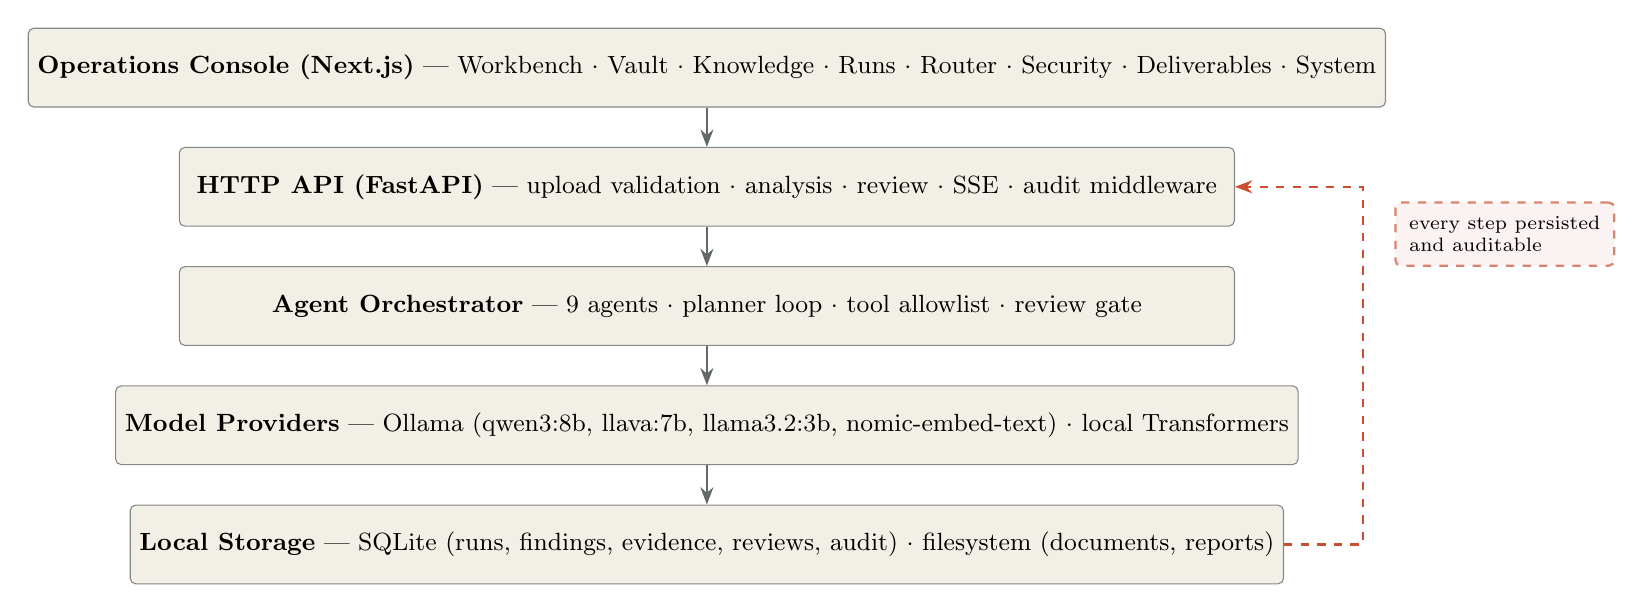
\begin{tikzpicture}[node distance=5mm]
\node[layer] (ui)    {\textbf{Operations Console (Next.js)} --- Workbench $\cdot$ Vault $\cdot$ Knowledge $\cdot$ Runs $\cdot$ Router $\cdot$ Security $\cdot$ Deliverables $\cdot$ System};
\node[layer, below=of ui]    (api)    {\textbf{HTTP API (FastAPI)} --- upload validation $\cdot$ analysis $\cdot$ review $\cdot$ SSE $\cdot$ audit middleware};
\node[layer, below=of api]   (agents) {\textbf{Agent Orchestrator} --- 9 agents $\cdot$ planner loop $\cdot$ tool allowlist $\cdot$ review gate};
\node[layer, below=of agents](models) {\textbf{Model Providers} --- Ollama (qwen3:8b, llava:7b, llama3.2:3b, nomic-embed-text) $\cdot$ local Transformers};
\node[layer, below=of models](store)  {\textbf{Local Storage} --- SQLite (runs, findings, evidence, reviews, audit) $\cdot$ filesystem (documents, reports)};
\draw[arrow] (ui) -- (api);
\draw[arrow] (api) -- (agents);
\draw[arrow] (agents) -- (models);
\draw[arrow] (models) -- (store);
\draw[oarrow, dashed] (store.east) -- ++(1.0,0) |- node[note, right, xshift=4mm, yshift=-6mm] {every step persisted\\ and auditable} (api.east);
\end{tikzpicture}
\caption{Layered architecture. All processing stays on the host.}
\end{figure}

\subsection{Agent Catalogue}
Nine agents share one \texttt{RunContext} and append structured steps, so a run
leaves a complete trace.

\begin{table}[htbp]
\centering
\small
\begin{tabular}{@{}p{0.4cm} p{3.1cm} p{8.6cm}@{}}
\toprule
\textbf{\#} & \textbf{Agent} & \textbf{Responsibility} \\
\midrule
1 & Security & Confirms air-gapped mode and that the active provider is local; blocks external providers. \\
2 & Router & Keyword-based task classification (vision / code / extraction / classification / reasoning) and model selection. \\
3 & Document & Loads documents; extracts text locally from TXT, CSV, PY, DOCX, and PDF. \\
4 & Vision & Inspects supplied images using a local vision model in every analysis mode; observations are separate from OCR fields and no prepared regions are emitted. \\
5 & Knowledge & RAG retrieval over the local index; indexes an uploaded document for its run. \\
6 & Reasoning & Produces profile-based findings, advisory summaries, or literal field extractions. \\
7 & Verification & Re-checks every quoted excerpt against the source text and flags unsupported findings. \\
8 & Deliverable & Writes reports: TXT and Markdown always; DOCX, XLSX, PDF when libraries are present. \\
9 & Planner & Agentic mode: chooses the next eligible action from the tool allowlist, step by step. \\
\bottomrule
\end{tabular}
\caption{The nine agents. Supporting components: orchestrator, tool registry (6 tools), and review gate.}
\end{table}

\subsection{Pipeline Flow}
\begin{figure}[htbp]
\centering
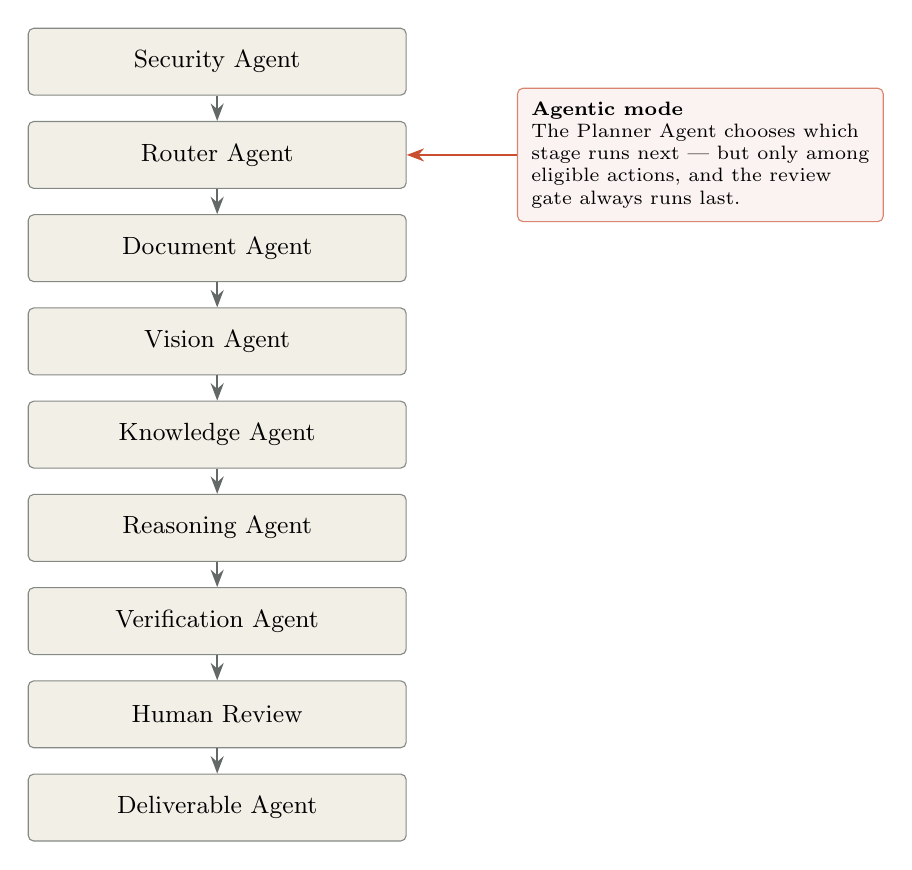
\begin{tikzpicture}[node distance=3.2mm]
\node[stage] (sec) {Security Agent};
\node[stage, below=of sec] (rtr) {Router Agent};
\node[stage, below=of rtr] (doc) {Document Agent};
\node[stage, below=of doc] (vis) {Vision Agent};
\node[stage, below=of vis] (kb)  {Knowledge Agent};
\node[stage, below=of kb]  (rea) {Reasoning Agent};
\node[stage, below=of rea] (ver) {Verification Agent};
\node[stage, below=of ver] (rev) {Human Review};
\node[stage, below=of rev] (del) {Deliverable Agent};
\foreach \a/\b in {sec/rtr,rtr/doc,doc/vis,vis/kb,kb/rea,rea/ver,ver/rev,rev/del}
  \draw[arrow] (\a) -- (\b);
\node[note, right=14mm of rtr] (plan) {\textbf{Agentic mode}\\ The Planner Agent chooses which\\ stage runs next --- but only among\\ eligible actions, and the review\\ gate always runs last.};
\draw[oarrow] (plan.west) -- (rtr.east);
\end{tikzpicture}
\caption{Fixed pipeline (left) and the planner's role in agentic runs (callout).}
\end{figure}

\subsection{Technology Stack}
\begin{table}[htbp]
\centering
\small
\begin{tabular}{@{}p{3.2cm} p{11cm}@{}}
\toprule
\textbf{Layer} & \textbf{Technology} \\
\midrule
Frontend & Next.js 14, React 18, TypeScript, Tailwind CSS \\
Backend & Python 3.10+, FastAPI, Pydantic, SQLite (stdlib \texttt{sqlite3}) \\
RAG & chunking, local embeddings, in-memory cosine similarity \\
Text extraction & \texttt{pypdf} (PDF), \texttt{python-docx} (DOCX), plain read (TXT/CSV/PY) \\
Inference & Ollama (host default) or local Transformers; explicit availability errors \\
Reporting & \texttt{fpdf2}/\texttt{reportlab} (PDF), \texttt{python-docx} (DOCX), \texttt{openpyxl} (XLSX) \\
System metrics & \texttt{nvidia-smi} (GPU), \texttt{psutil} (CPU/RAM), unavailable readings are null \\
Packaging & Docker, Docker Compose \\
\bottomrule
\end{tabular}
\caption{Technology stack.}
\end{table}

% ============================================================================
% 4. IMPLEMENTATION
% ============================================================================
\section{Implementation}

\subsection{Backend and Persistence}
The FastAPI backend exposes the HTTP API and persists all state to SQLite:
documents, tasks, agent runs, steps, findings, evidence, reviews, models,
audit logs, and deliverables. Connections are short-lived with
\texttt{row\_factory} set for dict-like access, so the app runs without an ORM
dependency. Deliverable files are written to the local \texttt{generated/}
directory.

\subsection{Document Ingestion and Text Extraction}
Uploads are validated against an extension allowlist
(\texttt{pdf, png, jpg, jpeg, txt, docx, csv, py}), a 25~MB size cap, and a
path-traversal-safe filename sanitiser; an upload never overwrites an earlier
file. Text extraction is performed locally: PDF pages via \texttt{pypdf},
DOCX paragraphs via \texttt{python-docx}, and plain reads for TXT, CSV, and PY.
Page breaks are preserved so a finding can be traced to its page. If a format
has no extractor (for example a PNG), the run records a clear note instead of
failing.

\subsection{Domain Profiles and Analysis Modes}
Analysis is profile-based rather than tied to one facility type.

\begin{table}[htbp]
\centering
\small
\begin{tabular}{@{}p{3.4cm} p{4.6cm} p{6.2cm}@{}}
\toprule
\textbf{Profile} & \textbf{Intended content} & \textbf{Review vocabulary} \\
\midrule
General documents & Reports, policies, correspondence, records & issues, delays, missing items, exceptions, risks \\
Industrial engineering & Equipment integrity, maintenance, process safety & corrosion, leaks, vibration, fouling, equipment terms \\
\bottomrule
\end{tabular}
\caption{Built-in profiles. Vocabulary lives in \texttt{backend/app/domains/profiles.py}.}
\end{table}

\begin{table}[htbp]
\centering
\small
\begin{tabular}{@{}p{3.0cm} p{11.2cm}@{}}
\toprule
\textbf{Mode} & \textbf{Behaviour} \\
\midrule
Risk review & Finds sentences matching the profile vocabulary; each finding quotes its source and is re-checked by the verification agent. Confidence reflects match strength, not a probability. \\
Summary & Model-generated advisory summary of extracted text; for images, the vision model describes visible content. Verification is marked not applicable. \\
Extract fields & Deterministic extraction of dates, equipment identifiers, and measurements, each with an exact source excerpt. \\
\bottomrule
\end{tabular}
\caption{Analysis modes for uploaded documents.}
\end{table}

\subsection{Retrieval-Augmented Generation}
Text is chunked on word boundaries (approximately 480 characters with 80
characters of overlap). Each chunk is embedded and stored in an in-memory
index. Queries are embedded the same way and ranked by cosine similarity;
non-positive similarities are discarded. The embedding backend is selected at
runtime: Ollama \texttt{nomic-embed-text} when available, then Sentence
Transformers if installed, then the deterministic hash-embedding fallback.

\subsection{Local Model Routing}
Tasks are routed by keyword classification to role-specific local models.

\begin{table}[htbp]
\centering
\small
\begin{tabular}{@{}p{6.4cm} p{7.8cm}@{}}
\toprule
\textbf{Role} & \textbf{Default model} \\
\midrule
Reasoning and evidence synthesis & \texttt{qwen3:8b} \\
Vision and image description & \texttt{llava:7b} \\
Other text tasks and planner choices & \texttt{llama3.2:3b} \\
RAG embeddings & hash by default; \texttt{nomic-embed-text} when configured \\
\midrule
Model-free lexical retrieval & local hash embeddings \\
\bottomrule
\end{tabular}
\caption{Model role assignments (overridable by environment variables).}
\end{table}

\noindent If a model or the Ollama server is unavailable, model-dependent requests return an availability error. Source-term risk review continues with a warning if only advisory inference fails. In air-gapped
mode the Ollama URL must be loopback; any other host raises an
\texttt{AirgapViolation}.

\subsection{Agentic Planner and Guardrails}
In agentic mode the planner observes the run state and chooses one action per
step. Actions are backed by a fixed, read-only tool allowlist; there is no
dynamic registration and no shell, SQL, filesystem, or network tool.

\begin{table}[htbp]
\centering
\small
\begin{tabular}{@{}p{3.6cm} p{10.6cm}@{}}
\toprule
\textbf{Action} & \textbf{Eligible when} \\
\midrule
\texttt{inspect\_document} & Documents not loaded yet \\
\texttt{analyze\_pid} & Task mentions a diagram and regions not analysed \\
\texttt{search\_knowledge} & Nothing retrieved yet \\
\texttt{reason} & Evidence gathered, no findings yet \\
\texttt{verify} & Findings exist but are unverified \\
\texttt{human\_review} & Verification requires approval \\
\texttt{finish} & Everything above is complete \\
\bottomrule
\end{tabular}
\caption{Planner actions and their preconditions.}
\end{table}

\noindent\textbf{Guardrails} (enforced in code, covered by tests):
\begin{enumerate}[leftmargin=1.4em]
  \item \textbf{Bounded steps} --- \texttt{max\_steps} defaults to 10 with a
        hard cap of 20; hitting the limit halts the run.
  \item \textbf{Loop detection} --- repeating an action with identical
        arguments halts the run.
  \item \textbf{Tool allowlist} --- unknown tool names or unexpected arguments
        are rejected and halt the run.
  \item \textbf{Prerequisites} --- eligibility is computed from run state, so
        the planner cannot reason before gathering evidence or finish before
        verifying.
  \item \textbf{Review gate} --- always applied after the loop, independent of
        the planner.
  \item \textbf{Fail safe} --- any stop other than \texttt{finish} marks the
        run \texttt{halted} and escalates every finding to human review.
\end{enumerate}

\subsection{Human-in-the-Loop Review Gate}
A finding is held for human approval when any of the following is true:
severity is \emph{high} or \emph{critical}; it cites no evidence or a source
that is not in the knowledge base; confidence is below the configured
threshold (default 75); or it was never verified. Held runs end as
\texttt{awaiting\_review} and become \texttt{completed} only after a reviewer
approves or rejects each flagged finding through the API or the Agent Runs
page.

\subsection{Deliverable Generation}
Every run writes a text and Markdown report; DOCX, XLSX, and PDF variants are
added when the corresponding libraries are installed. Reports include the
selected profile and mode, the executive summary, findings with evidence
excerpts and page references, verification results, and the full pipeline
trace. Optional libraries are import-guarded, so the application starts and
degrades gracefully without them.

\subsection{Operations Console}
The Next.js console provides nine sections:
Overview, Workbench (analysis setup and stored-document execution), Document Vault
(upload and analyse), Knowledge Base (RAG search), Agent Runs (traces,
evidence, approve/reject), Model Router (assignments and rules), Security
Center (controls and live audit log), Deliverables (generated reports), and
System (live hardware metrics and service status). The console displays unavailable states when the backend is offline.

\subsection{System Monitoring}
The System page reports real hardware values when they can be detected: GPU
name, utilisation, temperature, and VRAM through \texttt{nvidia-smi}; CPU and
RAM through \texttt{psutil}. When detection is unavailable, the API returns null readings and the interface displays unavailable. No synthetic measurements are generated.

% ============================================================================
% 5. RESULTS AND TESTING
% ============================================================================
\section{Results and Testing}

\subsection{Automated Test Suite}
The backend suite comprises \textbf{114 tests} (\texttt{pytest}) and passes on
the development machine. Coverage areas:

\begin{table}[htbp]
\centering
\small
\begin{tabular}{@{}p{6.0cm} p{8.2cm}@{}}
\toprule
\textbf{Area} & \textbf{Representative checks} \\
\midrule
Planner loop and guardrails & step limit, loop detection, rogue tool calls, early-finish blocked by the review gate \\
Tool allowlist & unknown tools rejected; invalid or extra arguments rejected \\
Review gate and approvals & hold rules; run completes only after all flagged findings are decided \\
Model routing & role-to-model mapping; Ollama request formatting (including image payloads) \\
Profiles and modes & profile vocabularies differ; summary records no findings; field extraction cites sources; unknown profile/mode rejected (HTTP 422) \\
Knowledge search & ranked results; input validation \\
Air-gap guard & loopback-only inference URLs; external provider rejection \\
Uploaded-document analysis & extraction, excerpt verification, unreadable files, duplicate filenames, image handling without model calls \\
\bottomrule
\end{tabular}
\caption{Test coverage summary.}
\end{table}

\noindent Frontend validation: \texttt{npx tsc --noEmit} and
\texttt{npm run build} both complete successfully.

\subsection{Document Analysis Behaviour}
\begin{itemize}[leftmargin=1.4em]
  \item \textbf{Text documents} --- risk review returns findings that quote
        their source; the verification agent re-checks every excerpt and
        reports 100\% confirmation when excerpts are present.
  \item \textbf{Images} --- risk review uses locally extracted OCR text when available; without readable text it provides guidance; Every image mode uses the local vision model and records an
        advisory description.
  \item \textbf{Field extraction} --- dates, equipment identifiers, and
        measurements are extracted literally, each with its exact sentence.
\end{itemize}

\subsection{Live Hardware Metrics}
GPU readings are probed locally with \texttt{nvidia-smi}; CPU and RAM use \texttt{psutil}. Missing capabilities produce unavailable readings and do not fabricate a hardware profile.

% ============================================================================
% 6. SECURITY
% ============================================================================
\section{Security and Privacy}

\subsection{Implemented Controls}
\begin{itemize}[leftmargin=1.4em]
  \item \textbf{Air-gapped mode} (default): external providers are rejected
        and inference URLs must be loopback.
  \item \textbf{No cloud AI SDKs}: the backend makes no outbound AI call.
  \item \textbf{Upload controls}: extension allowlist, 25~MB cap,
        path-traversal-safe names, no overwrites.
  \item \textbf{Isolated code execution}: explicitly submitted Python runs in disposable local Linux containers with networking disabled, a non-root worker, resource limits, and bounded output. Document analysis does not execute uploaded code.
  \item \textbf{Planner guardrails} and the mandatory review gate
        (Section~4.6).
  \item \textbf{Local audit log}: uploads, analyses, runs, searches, reviews,
        and downloads are recorded in a local table and surfaced in the
        Security Center.
\end{itemize}

\subsection{Known Gaps (Prototype Scope)}
Stated plainly so the console is not mistaken for a production guarantee:
no authentication or role-based access control; no encryption at rest; the
audit log is not tamper-evident; Docker Compose does not isolate the container
network; the frontend fetches fonts at build time, so the build requires
internet access once.

% ============================================================================
% 7. LIMITATIONS
% ============================================================================
\section{Limitations}

\begin{itemize}[leftmargin=1.4em]
  \item \textbf{Risk review is profile-term extraction.} It can miss risks
        phrased without those terms, and its ``confidence'' is match strength,
        not a probability.
  \item \textbf{Model output does not authoritatively create findings yet.}
        Summaries and advisory analyses are recorded in the run trace;
        findings come from profile-term extraction or literal field
        extraction.
  \item \textbf{OCR requires local dependencies.} Tesseract extracts raster text and scanned PDF pages when installed. Low-confidence OCR requires review.
  \item \textbf{Profiles use explicit vocabularies.} The eight profiles are configurable vocabularies, not comprehensive domain
        expertise. Multi-document comparison is not implemented.
  \item \textbf{Model availability.} Ollama calls require the local service
        and the listed model tags; automated tests mock those calls.
\end{itemize}

% ============================================================================
% 8. CONCLUSION AND FUTURE SCOPE
% ============================================================================
\section{Conclusion and Future Scope}

\projectname{} demonstrates that a confidential document-analysis workflow can
be built entirely on local infrastructure with meaningful safety properties:
grounded findings, verified citations, explicit domain profiles, a bounded
agentic planner, and a human approval gate. The system is implemented end to
end --- from upload and extraction through retrieval, analysis, verification,
review, and report generation --- and is covered by an automated test suite.

\noindent\textbf{Future scope:}
\begin{itemize}[leftmargin=1.4em]
  \item Use validated model output to produce structured findings while
        preserving evidence checks and human review.
  \item Add real OCR and P\&ID symbol/tag detection.
  \item Extend the planner to uploaded documents and deliverable generation.
  \item Persistent vector store with hybrid (dense + keyword) retrieval.
  \item Additional domain profiles (procurement, compliance, legal).
  \item Multi-document comparison and cross-reference workflows.
  \item Authentication, RBAC, encryption at rest, and a hash-chained audit
        log.
  \item Network-isolated deployment packaging for a true physical air gap.
\end{itemize}

% ============================================================================
% REFERENCES
% ============================================================================
\begin{thebibliography}{9}
\bibitem{rag} P. Lewis et al., ``Retrieval-Augmented Generation for
Knowledge-Intensive NLP Tasks,'' \emph{Advances in Neural Information
Processing Systems}, 2020.
\bibitem{react} S. Yao et al., ``ReAct: Synergizing Reasoning and Acting in
Language Models,'' \emph{International Conference on Learning Representations},
2023.
\bibitem{ollama} Ollama, ``Run LLMs locally.'' [Online].
Available: \url{https://ollama.com}
\bibitem{fastapi} S. Ram\'irez, ``FastAPI.'' [Online].
Available: \url{https://fastapi.tiangolo.com}
\bibitem{nextjs} Vercel, ``Next.js.'' [Online].
Available: \url{https://nextjs.org}
\bibitem{sqlite} SQLite Consortium, ``SQLite.'' [Online].
Available: \url{https://sqlite.org}
\bibitem{psutil} G. Rodola, ``psutil: Cross-platform process and system
utilities.'' [Online]. Available: \url{https://github.com/giampaolo/psutil}
\bibitem{nvidia} NVIDIA, ``nvidia-smi.'' [Online].
Available: \url{https://developer.nvidia.com/nvidia-system-management-interface}
\end{thebibliography}

% ============================================================================
% APPENDIX A - API REFERENCE
% ============================================================================
\appendix
\section{API Reference}
\begin{longtable}{@{}p{1.6cm} p{6.4cm} p{6.4cm}@{}}
\toprule
\textbf{Method} & \textbf{Path} & \textbf{Purpose} \\
\midrule
\endfirsthead
\toprule
\textbf{Method} & \textbf{Path} & \textbf{Purpose} \\
\midrule
\endhead
GET & \texttt{/api/health} & Status, mode, version \\
GET & \texttt{/api/system/status} & Measured GPU/CPU/RAM or null, models, vector DB, sandbox, network \\
GET & \texttt{/api/profiles} & Document profiles and analysis modes \\
POST & \texttt{/api/documents/upload} & Upload a file (allowlist, 25~MB cap, sanitised name) \\
GET & \texttt{/api/documents} $\cdot$ \texttt{/api/documents/\{id\}} & List / fetch documents \\
POST & \texttt{/api/documents/\{id\}/analyze} & Analyse with \texttt{profile} and \texttt{analysis\_mode} \\
POST & \texttt{/api/tasks} & Create a task using a required document ID \\
GET & \texttt{/api/agent/tools} & Planner tool allowlist \\
POST & \texttt{/api/agent/run} & Bounded agentic planner run \\
GET & \texttt{/api/agents/runs} $\cdot$ \texttt{/api/agents/runs/\{id\}} & Run list / full trace \\
POST & \texttt{/api/review/\{id\}/approve} $\cdot$ \texttt{/reject} & Human review decision \\
GET & \texttt{/api/models} & Model catalogue, routing rules, providers \\
GET & \texttt{/api/knowledge} $\cdot$ POST \texttt{/api/knowledge/search} & Knowledge-base stats / RAG search \\
GET & \texttt{/api/audit-logs} & Audit entries \\
GET & \texttt{/api/deliverables} $\cdot$ \texttt{/api/deliverables/\{id\}/download} & List / download reports \\
\bottomrule
\end{longtable}

\noindent Interactive API documentation is served at
\texttt{http://localhost:8000/docs}.

% ============================================================================
% APPENDIX B - SETUP
% ============================================================================
\section{Setup and Configuration}

\begin{lstlisting}[language=bash, caption={Local development (host defaults to local Ollama).}]
# 1. Local models (optional but recommended)
ollama pull qwen3:8b
ollama pull llava:7b
ollama pull llama3.2:3b
ollama pull nomic-embed-text

# 2. Backend
cd backend
python -m venv .venv && .venv\Scripts\activate   # Windows
pip install -r requirements.txt
python -m uvicorn app.main:app --port 8000       # http://localhost:8000/docs

# 3. Frontend (second terminal)
cd frontend
npm install
npm run dev                                      # http://localhost:3000
\end{lstlisting}

\begin{lstlisting}[language=bash, caption={Local lexical retrieval without an embedding model.}]
KAVACH_EMBEDDING_BACKEND=hash
\end{lstlisting}

\begin{table}[htbp]
\centering
\small
\begin{tabular}{@{}p{5.4cm} p{3.4cm} p{5.4cm}@{}}
\toprule
\textbf{Variable} & \textbf{Default} & \textbf{Purpose} \\
\midrule
\texttt{KAVACH\_MODE} & \texttt{airgapped} & Blocks external providers and non-loopback URLs \\
\texttt{KAVACH\_INFERENCE\_PROVIDER} & \texttt{ollama} & \texttt{ollama} or \texttt{transformers} \\
\texttt{OLLAMA\_REASONING\_MODEL} & \texttt{qwen3:8b} & Reasoning model \\
\texttt{OLLAMA\_VISION\_MODEL} & \texttt{llava:7b} & Image model \\
\texttt{OLLAMA\_OTHER\_MODEL} & \texttt{llama3.2:3b} & Other text tasks and planner choices \\
\texttt{OLLAMA\_EMBED\_MODEL} & \texttt{nomic-embed-text} & RAG embeddings \\
\texttt{KAVACH\_PLANNER\_MAX\_STEPS} & \texttt{10} & Planner step budget (hard cap 20) \\
\texttt{KAVACH\_REVIEW\_MIN\_CONFIDENCE} & \texttt{75} & Findings below this need approval \\
\texttt{KAVACH\_MAX\_UPLOAD\_MB} & \texttt{25} & Upload size cap \\
\bottomrule
\end{tabular}
\caption{Key environment variables (see \texttt{.env.example}).}
\end{table}

\end{document}
